\documentclass[10pt,aspectratio=43,mathserif]{beamer}		
%设置为 Beamer 文档类型,设置字体为 10pt,长宽比为16:9,数学字体为 serif 风格

%%%%-----导入宏包-----%%%%
\usepackage{seu}
\usepackage{xeCJK}
\usepackage{amsmath,amsfonts,amssymb,bm}
\usepackage{color}
\usepackage{graphicx,hyperref,url}
\usepackage{booktabs}
\renewcommand{\thempfootnote}{\arabic{mpfootnote}}
%%%%%%%%%%%%%%%%%%


%%%%-----设置字体-----%%%%
%Windows和Mac OS下都可用
\setsansfont[Path=fonts/]{Helvetica}

%\setsansfont{Times New Roman}

%仅Windows可用
%\setCJKmainfont{Hiragino Sans GB W3}

%仅Mac OS下可用
%\setCJKmainfont{Songti SC}




%设置 Beamer 主题
\beamertemplateballitem


\AtBeginSection[]
{
  \begin{frame}<beamer>
    \frametitle{\textbf{目录}}
    \textbf{\tableofcontents[currentsection]}
  \end{frame}
}

%%%%----首页信息设置----%%%%
%%%%----标题设置
\title[高光谱图像的非凸低秩表示]{
	\fontsize{14pt}{25pt}\selectfont \textbf{高光谱图像的非凸低秩表示}
}
\subtitle{\fontsize{13pt}{14pt}\selectfont {在图像降噪方面的使用}}			
%%%%----机构信息
\institute[SEU]{
	\fontsize{10pt}{11pt}\selectfont {东南大学{\quad}吴健雄学院}
}
%%%%----个人信息设置
\author[陈安皓]{
	\fontsize{13pt}{14pt}\selectfont {学生姓名:陈安皓}\\
	\fontsize{13pt}{14pt}\selectfont {指导教师:贾育衡}
}
%%%%----日期信息
\date[2021年6月8日]{
 2021年6月8日
}

\begin{document}
%生成标题页
\begin{frame}
\titlepage
\end{frame}

\section*{目录}

%\begin{frame}
%\frametitle{\textbf{目录}}
%\textbf{\tableofcontents}
%\end{frame}

\section[引言]{引言}

\begin{frame}
\frametitle{\textbf{背景知识}}
\begin{block}{\textbf{高光谱图像及其成像原理}}
% 插入图片
\begin{figure}[H]
\centering
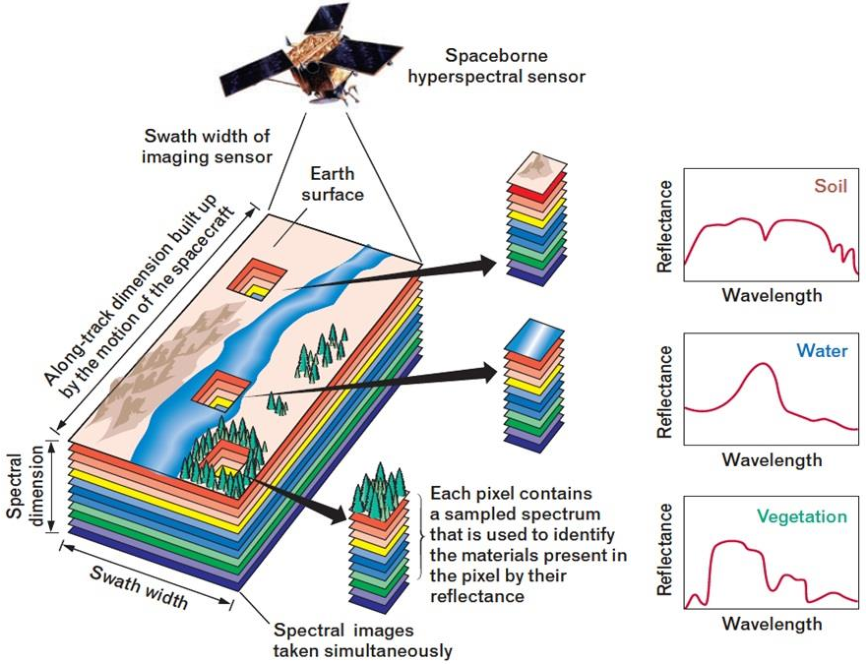
\includegraphics[scale=0.22]{img-principleofphotograph.png}
\caption{高光谱图像的成像原理\footnote{图片来源:semanticscholar.org}}
\end{figure}
\end{block}
\end{frame}
    
\begin{frame}
\frametitle{\textbf{背景知识}}
\begin{block}{\textbf{高光谱图像的特征}}
% 插入图片
\begin{figure}[H]
\centering
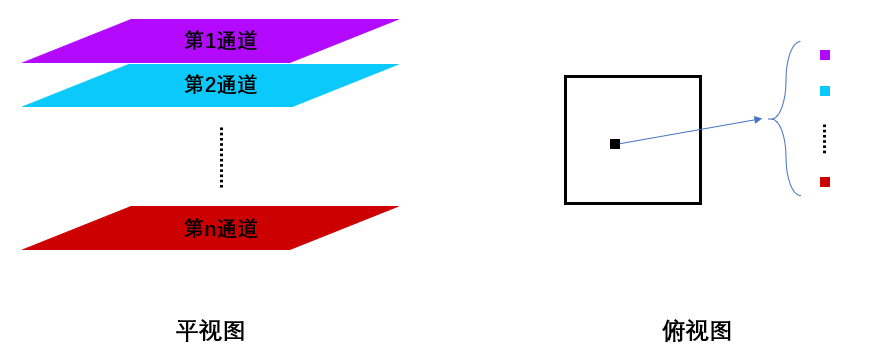
\includegraphics[scale=0.5]{img-characterofphotograph.png}
\caption{高光谱图像的特征}
\end{figure}
\end{block}
    	
\begin{block}{\textbf{高光谱图像的部分应用领域}}
$\bullet$农业 \qquad 
$\bullet$军事 \qquad 
$\bullet$环境 \qquad 
$\bullet$地学
\end{block}
\end{frame}

%\section[相关工作]{相关工作}
%\begin{frame}
%\frametitle{\textbf{相关工作}}
%
%\end{frame}

\section[研究路线]{研究路线}
\begin{frame}
\frametitle{\textbf{问题建模}}
\par 假设一幅一维图像$Y$受到噪声的污染,即:
\begin{displaymath}
Y = X + N
\end{displaymath}
式中,
\par$X$代表未受到污染的、干净的图像,$X \in \mathbb{R}^{m \times n}$;
\par$N$代表噪声,$N \in \mathbb{R}^{m \times n}$;
\par$Y$代表成像设备获取到的图像,即受到污染的图像,$Y \in \mathbb{R}^{m \times n}$。
\newline
\par 那么,图像降噪的工作就是将$Y$复原为$X$。
\end{frame}

\begin{frame}
\frametitle{\textbf{问题建模}}
\begin{block}{\textbf{自然图像的低秩性}}
\begin{columns}
\column{.5\textwidth}
\begin{figure}[!t]
\centering
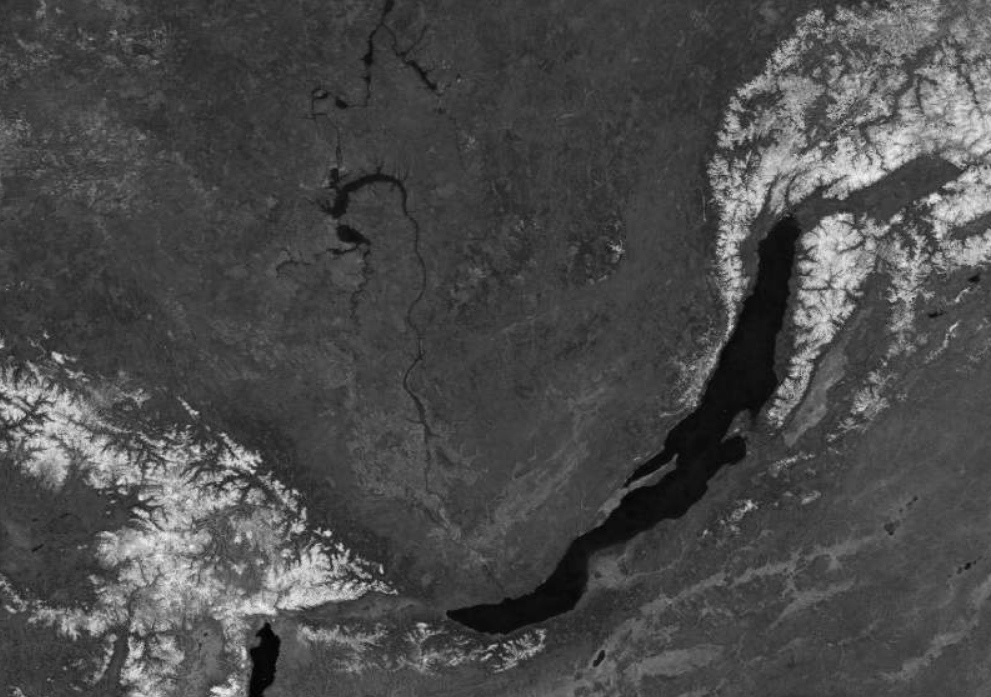
\includegraphics[scale=0.12]{x.png}
\caption{一张自然图像}
\label{example-figure}
\end{figure}

\column{.5\textwidth}
\begin{figure}[!t]
\centering
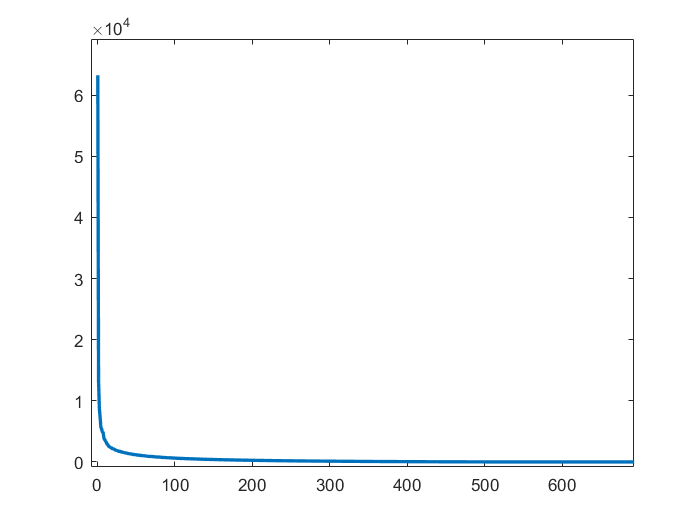
\includegraphics[scale=0.21]{y.png}
\caption{图\ref{example-figure}的奇异值分布图}
\label{example-figure-svd}
\end{figure}
\end{columns}
\end{block}
\par 基于低秩假设的图像降噪方法可以被形式化为
\begin{displaymath}
arg\min\limits_{X} \quad rank(X)
\end{displaymath}
\end{frame}

\begin{frame}
\frametitle{\textbf{问题建模}}
\par 在对图像进行降噪处理时,既需要去除图像里的噪声,同时也需要尽可能地保留原来的信息。因此,实际上,需要求解的最优化问题是
\begin{equation}
\centering
arg\min\limits_{X} \quad \left\|Y-X\right\|_F^2 + \lambda \cdot rank(X)
\label{F-rank}
\end{equation}
式中,
\par$X$代表未受到污染的、干净的图像,$X \in \mathbb{R}^{m \times n}$;
\par$N$代表噪声,$N \in \mathbb{R}^{m \times n}$;
\par$Y$代表成像设备获取到的图像,即受到污染的图像,$Y \in \mathbb{R}^{m \times n}$;
\par$\left\|*\right\|_F$表示$Frobenius$范数;
\par$\lambda$是正则化参数。

\end{frame}

\begin{frame}
\frametitle{\textbf{用(普通)核范数替代秩函数}}
\par 然而,式\ref{F-rank}
\begin{displaymath}
arg\min\limits_{X} \quad \left\|Y-X\right\|_F^2 + \lambda \cdot {\color{red}{rank(X)}}
\end{displaymath}
\par 是一个NP-hard问题。
\newline
\newline
\par 通常使用秩函数的凸近似,也就是核范数,作为式\ref{F-rank}中秩函数的替代:
\begin{equation}
\centering
arg\min\limits_{X} \quad \left\|Y-X\right\|_F^2 + \lambda \cdot {\color{red}{\left\|X\right\|_*}}
\label{F-NN}
\end{equation}
式中,
\par $\left\|*\right\|_*$表示核范数。
\par $\left\|X\right\|_* = \sum\limits_{i=1}^{n}\sigma_i(X)$,$\sigma_i(X)$表示矩阵$X$的第$i$个奇异值。
\end{frame}

\begin{frame}
\frametitle{\textbf{用截断式核范数替代秩函数}}
\begin{columns}
\column{.55\textwidth}
\par 式\ref{F-rank}
\begin{displaymath}
arg\min\limits_{X} \quad \left\|Y-X\right\|_F^2 + \lambda \cdot {\color{red}{rank(X)}}
\end{displaymath}
\par 更新为
\begin{equation}
\centering
arg\min\limits_{X} \quad \left\|Y-X\right\|_F^2 + \lambda \cdot {\color{red}{\left\|X\right\|_{tr,*}}}
\label{F-TNN}
\end{equation}
式中,
\par $\left\|*\right\|_{tr,*}$表示截断式核范数。
\par $\left\|X\right\|_{tr,*} = \sum\limits_{i=r+1}^{n}\sigma_i(X)$

\column{.45\textwidth}
\begin{figure}[!t]
\centering
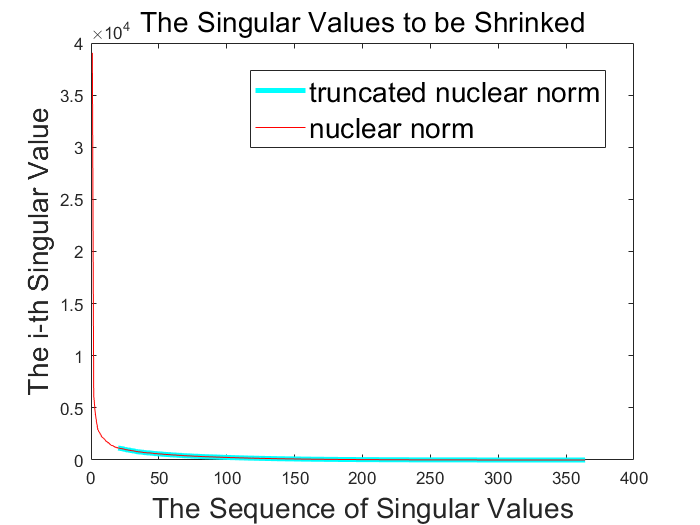
\includegraphics[scale=0.3]{surrogate-to-rank-2.png}
\caption{截断式核范数的几何意义(取$r=19$)}
\label{surrogate-to-rank-2}
\end{figure}
\end{columns}
\end{frame}

\begin{frame}
\frametitle{\textbf{用权重式核范数替代秩函数}}
\par 式\ref{F-rank}
\begin{displaymath}
arg\min\limits_{X} \quad \left\|Y-X\right\|_F^2 + \lambda \cdot {\color{red}{rank(X)}}
\end{displaymath}
\par 更新为
\begin{equation}
\centering
arg\min\limits_{X} \quad \left\|Y-X\right\|_F^2 + \lambda \cdot {\color{red}{\left\|X\right\|_{w,*}}}
\label{F-WNN}
\end{equation}
式中,
\par $\left\|*\right\|_{w,*}$表示权重式核范数。
\par $\left\|X\right\|_{w,*} = \sum\limits_{i=1}^{n}w_i\sigma_i(X)$
\end{frame}

\begin{frame}
\frametitle{\textbf{用$log$-核范数替代秩函数}}
\begin{columns}
\column{.55\textwidth}
\par 式\ref{F-rank}
\begin{displaymath}
arg\min\limits_{X} \quad \left\|Y-X\right\|_F^2 + \lambda \cdot {\color{red}{rank(X)}}
\end{displaymath}
\par 更新为
\begin{equation}
\centering
arg\min\limits_{X} \quad \left\|Y-X\right\|_F^2 + \lambda \cdot {\color{red}{\left\|X\right\|_{log,*}}}
\label{F-LNN}
\end{equation}
式中,
\par $\left\|*\right\|_{log,*}$表示$log$-核范数。
\par $\left\|X\right\|_{log,*} = \sum\limits_{i=1}^{n}log(\sigma_i(X)+1)$

\column{.45\textwidth}
\begin{figure}[!t]
\centering
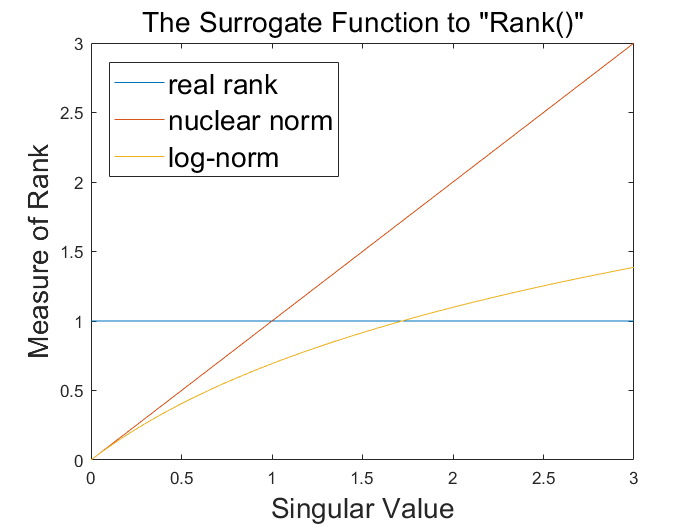
\includegraphics[scale=0.3]{surrogate-to-rank-1.png}
\caption{$log$-核范数的几何意义}
\label{surrogate-to-rank-1}
\end{figure}
\end{columns}
\end{frame}

\begin{frame}
\frametitle{\textbf{秩函数的其他放缩}}
\begin{columns}
\column{.6\textwidth}
\begin{table}[H]
\centering
\caption{秩函数的不同放缩(部分)}
\label{relaxation}
	
\begin{tabular}{c c}
\toprule
{\small{名称}}&{\small{表达式}}\\
\toprule
{\small{核范数}}&{\small{$\sum\limits_{i=1}^{n}\sigma_i$}}\\
\hline
{\small{截断式核范数}}&{\small{$\sum\limits_{i=r+1}^{n}\sigma_i$}}\\
\hline
{\small{权重式核范数}}&{\small{$\sum\limits_{i=1}^{n}w_i\sigma_i$}}\\
\hline
{\small{阀值式核范数}}&{\small{$\sum\limits_{i=r+1}^{n}min(\sigma_i, \theta)$}}\\
\hline
{\small{$log$-核范数}}&{\small{$\sum\limits_{i=1}^{n}log(\sigma_i+1)$}}\\
\hline
{\small{$\gamma$-核范数}}&{\small{$\sum\limits_{i=1}^{n}\cfrac{(1+\gamma)\sigma_i}{\gamma+\sigma_i}$}}\\
\hline
{\small{格曼}}&{\small{$\sum\limits_{i=1}^{n}\cfrac{\sigma_i}{\sigma_i + \gamma}$}}\\
%\hline
%{\small{拉普拉斯}}&{\small{$\sum\limits_{i=1}^{n}\left(1-exp(-\cfrac{\sigma_i}{\gamma})\right)$}}\\
\bottomrule
\end{tabular}
\end{table}
\column{.4\textwidth}
\par 表\ref{relaxation}列举了秩函数的几种替代(surrogate),或称放缩(relaxation)。它们可以被统一成:
\begin{displaymath}
rank(X) \approx \sum\limits_{i=1}^{n}f(\sigma_i(X))
\end{displaymath}
\end{columns}
\end{frame}

\section[实验]{实验}
\begin{frame}
\frametitle{\textbf{实验数据}}
\begin{columns}
	
\column{.25\textwidth}
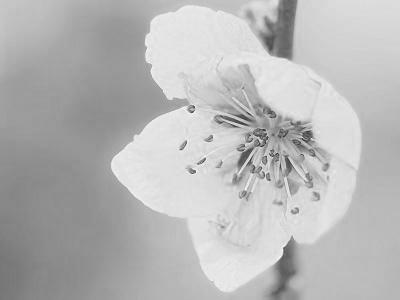
\includegraphics[scale=0.2]{exp-0.jpg}

\includegraphics[scale=0.2]{exp-4.jpg}
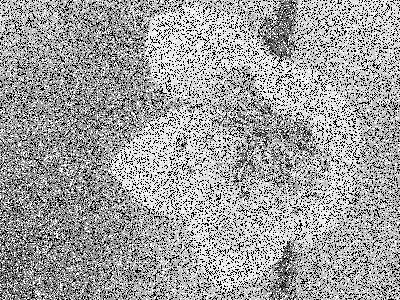
\includegraphics[scale=0.2]{exp-8.jpg}

\column{.25\textwidth}
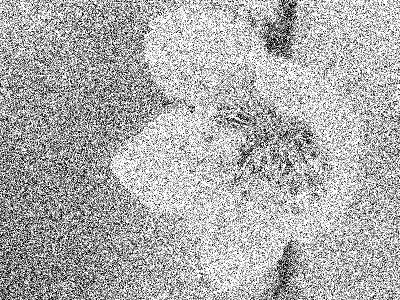
\includegraphics[scale=0.2]{exp-1.jpg}
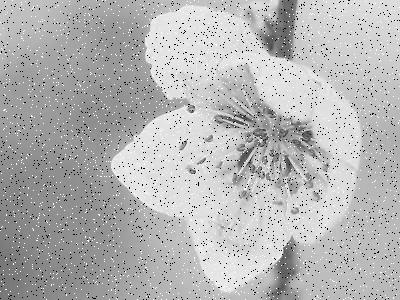
\includegraphics[scale=0.2]{exp-5.jpg}
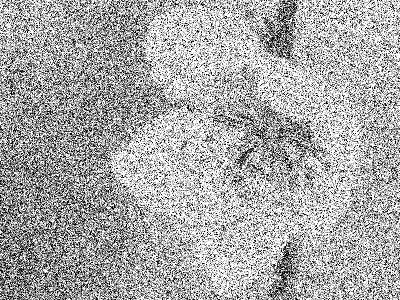
\includegraphics[scale=0.2]{exp-9.jpg}

\column{.25\textwidth}
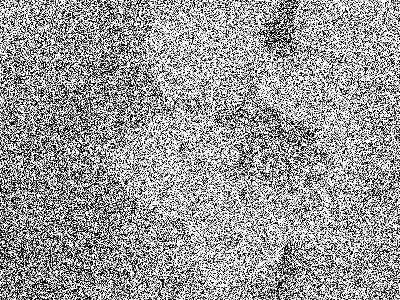
\includegraphics[scale=0.2]{exp-2.jpg}
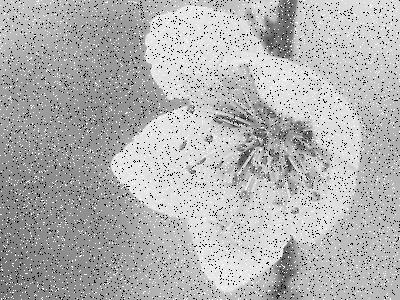
\includegraphics[scale=0.2]{exp-6.jpg}
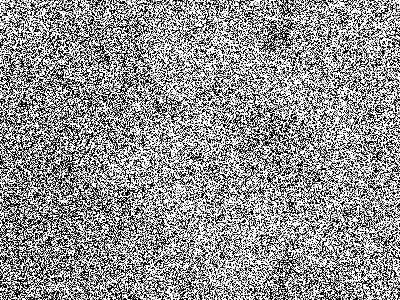
\includegraphics[scale=0.2]{exp-10.jpg}

\column{.25\textwidth}
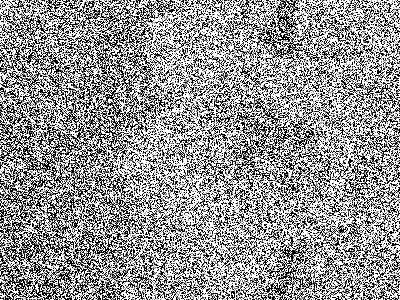
\includegraphics[scale=0.2]{exp-3.jpg}
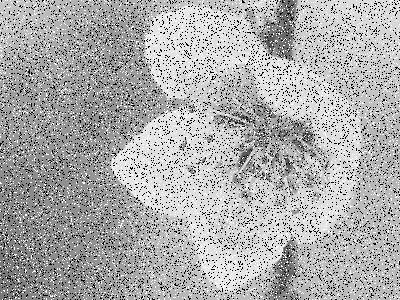
\includegraphics[scale=0.2]{exp-7.jpg}
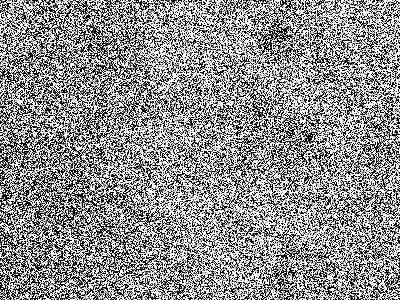
\includegraphics[scale=0.2]{exp-11.jpg}

\end{columns}
\end{frame}

\begin{frame}
\frametitle{\textbf{降噪效果展示(以权重式核范数为例)}}
\begin{columns}
\column{.5\textwidth}
\begin{figure}
\centering
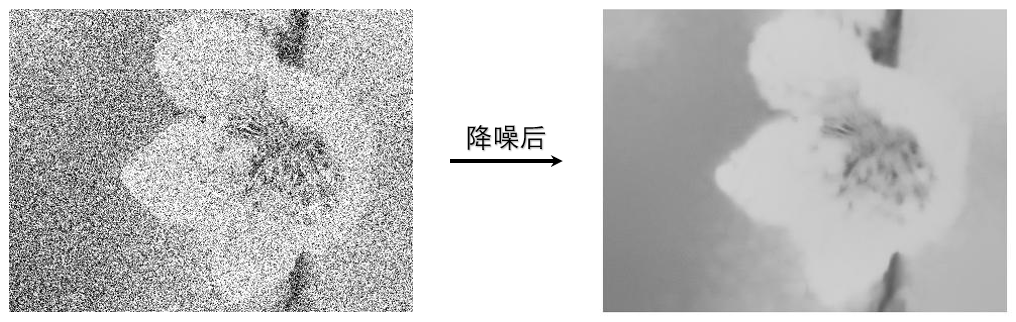
\includegraphics[scale=0.25]{Screenshot_1.png}
\caption{方差为0.1的零均值高斯噪声}
\end{figure}

\begin{figure}
\centering
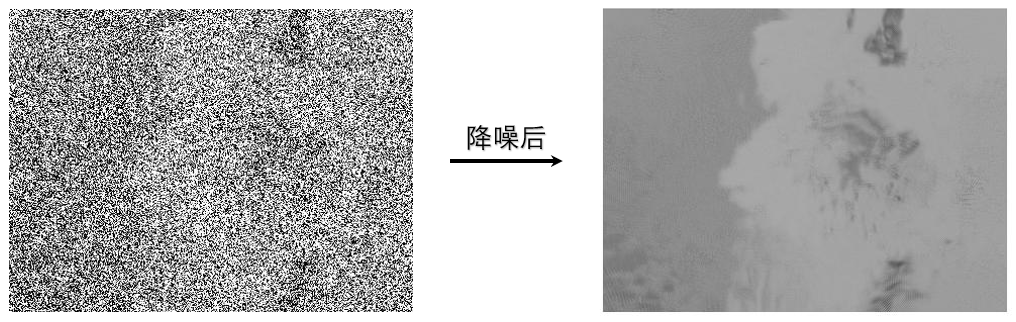
\includegraphics[scale=0.25]{Screenshot_3.png}
\caption{方差为1的零均值高斯噪声}
\end{figure}

\column{.5\textwidth}
\begin{figure}
\centering
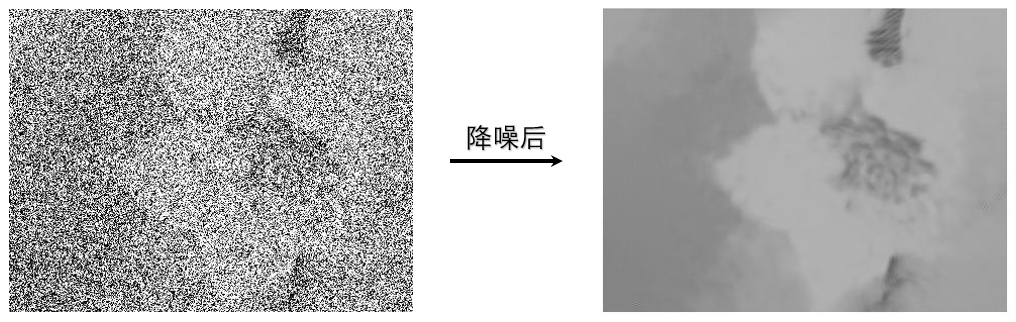
\includegraphics[scale=0.25]{Screenshot_2.png}
\caption{方差为0.5的零均值高斯噪声}
\end{figure}

\begin{figure}
\centering
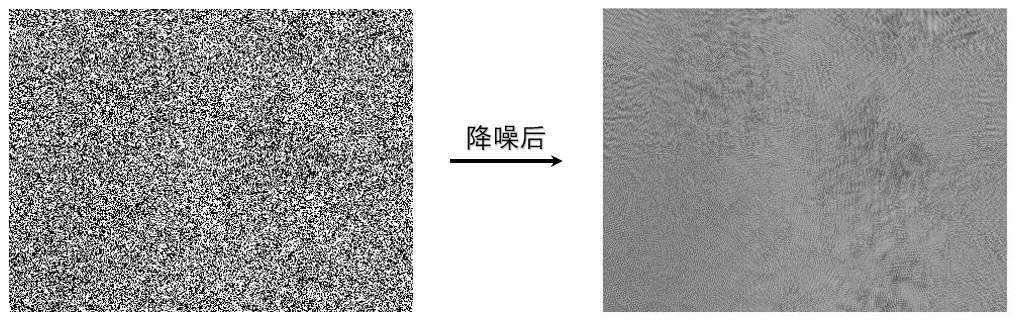
\includegraphics[scale=0.25]{Screenshot_4.png}
\caption{方差为5的零均值高斯噪声}
\end{figure}


\end{columns}
\end{frame}

\begin{frame}
\frametitle{\textbf{降噪效果展示(以权重式核范数为例)}}
\begin{columns}
\column{.5\textwidth}
\begin{figure}
\centering
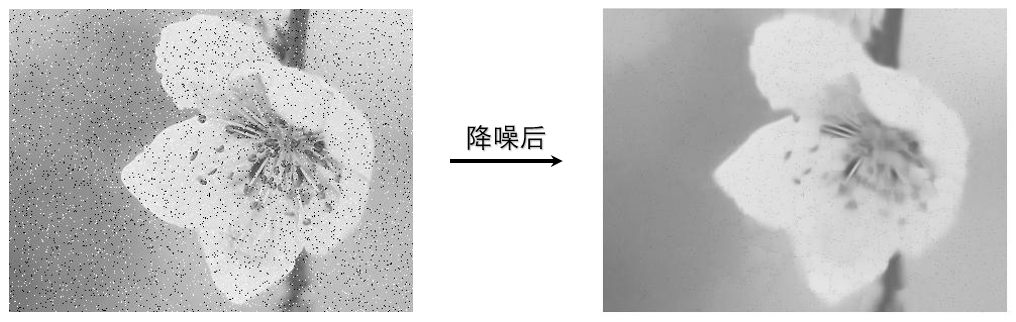
\includegraphics[scale=0.25]{Screenshot_5.png}
\caption{5\%椒盐噪声}
\end{figure}

\begin{figure}
\centering
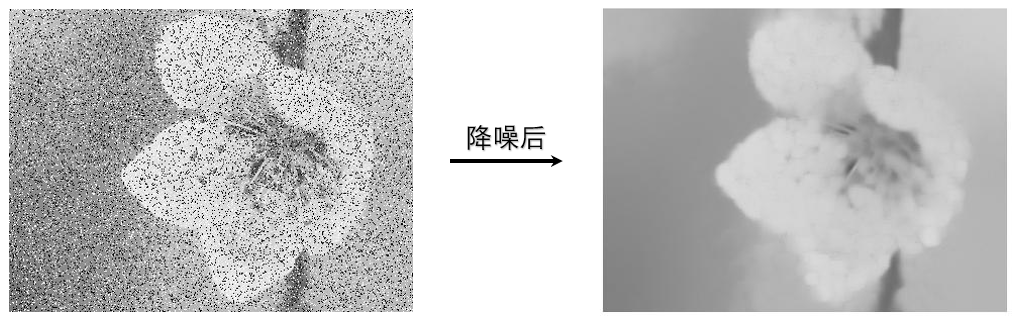
\includegraphics[scale=0.25]{Screenshot_7.png}
\caption{20\%椒盐噪声}
\end{figure}

\column{.5\textwidth}
\begin{figure}
\centering
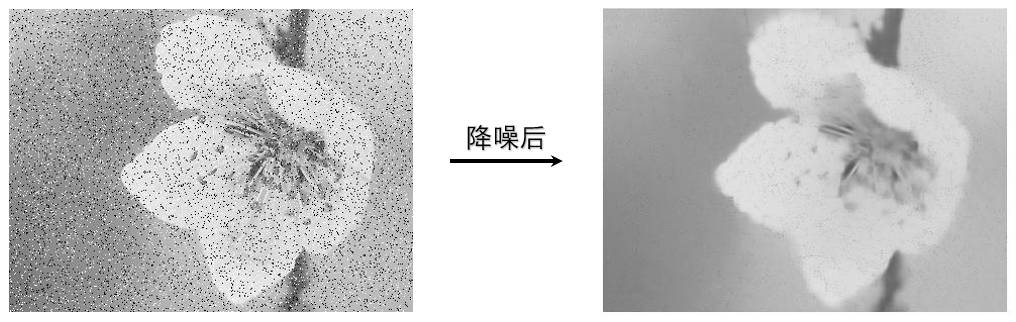
\includegraphics[scale=0.25]{Screenshot_6.png}
\caption{10\%椒盐噪声}
\end{figure}

\begin{figure}
\centering
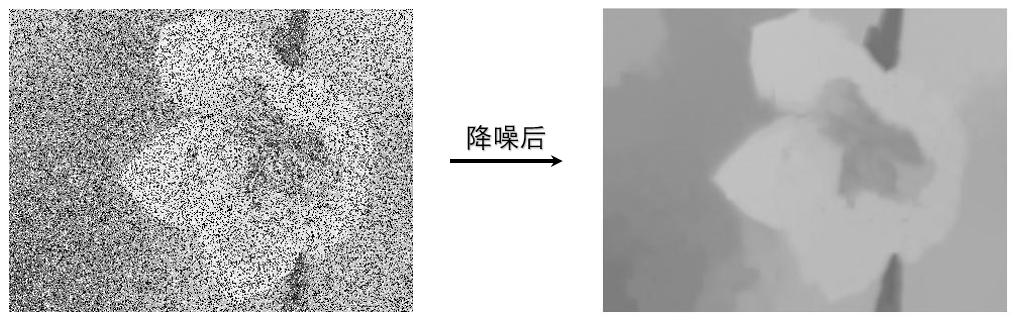
\includegraphics[scale=0.25]{Screenshot_8.png}
\caption{40\%椒盐噪声}
\end{figure}
	
\end{columns}
\end{frame}

\begin{frame}
\frametitle{\textbf{降噪效果展示(以权重式核范数为例)}}
\begin{columns}
\column{.5\textwidth}
\begin{figure}
\centering
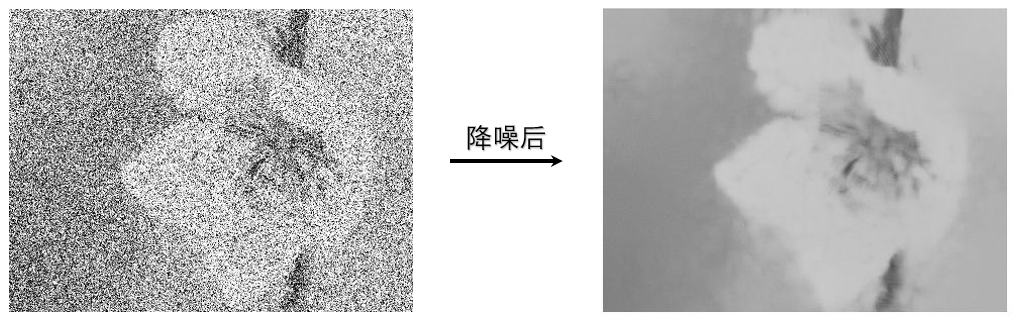
\includegraphics[scale=0.25]{Screenshot_9.png}
\caption{10\%椒盐+方差为0.1的零均值高斯噪声}
\end{figure}

\column{.5\textwidth}
\begin{figure}
\centering
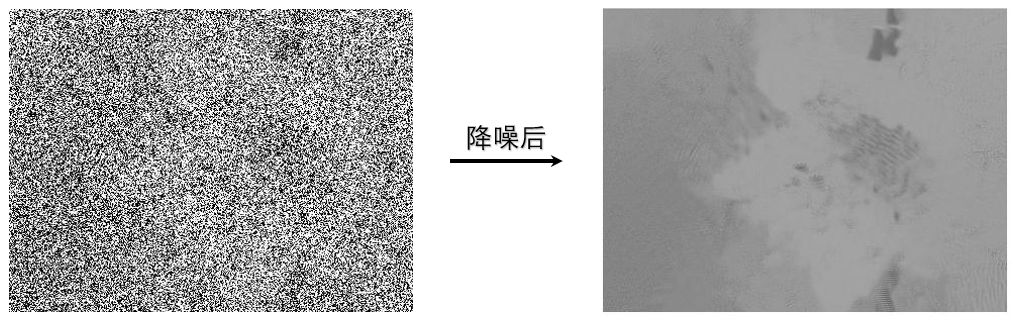
\includegraphics[scale=0.25]{Screenshot_10.png}
\caption{10\%椒盐+方差为1的零均值高斯噪声}
\end{figure}
\end{columns}
\begin{figure}
\centering
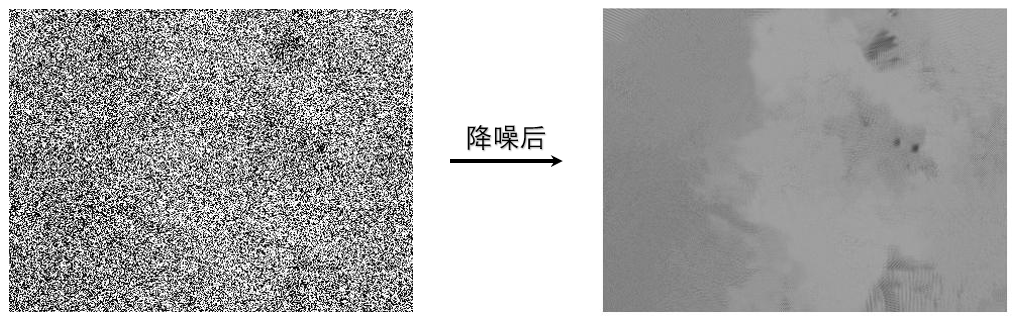
\includegraphics[scale=0.25]{Screenshot_11.png}
\caption{20\%椒盐+方差为1的零均值高斯噪声}
\end{figure}
\end{frame}

\begin{frame}
\frametitle{\textbf{不同降噪方法的降噪效果}}
\begin{columns}
\column{.5\textwidth}
\begin{figure}
\centering
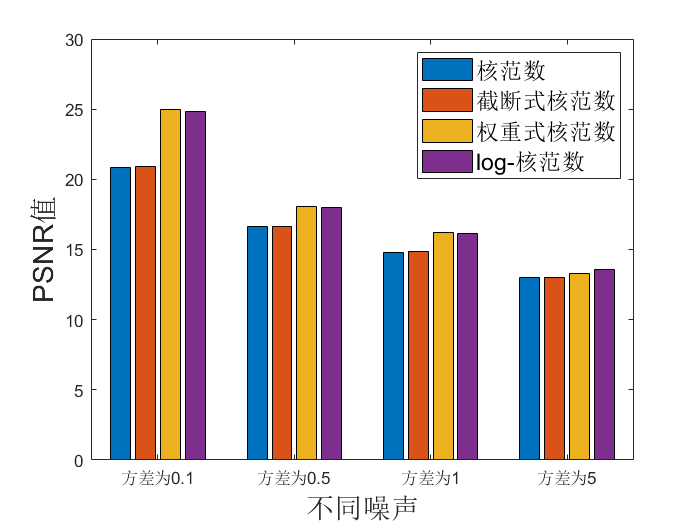
\includegraphics[scale=0.2]{exp-type-gaussian.png}
\caption{不同方差的零均值高斯噪声}
\end{figure}
\column{.5\textwidth}
\begin{figure}
\centering
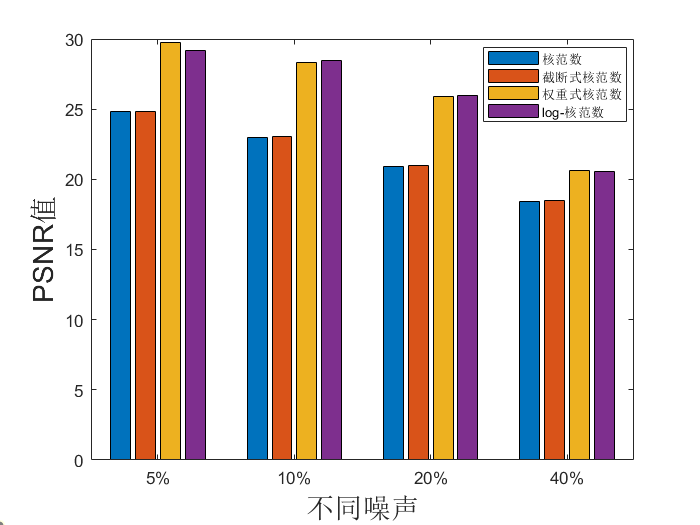
\includegraphics[scale=0.2]{exp-type-pepperandsalt.png}
\caption{不同程度的椒盐噪声}
\end{figure}
\end{columns}
\begin{figure}
\centering
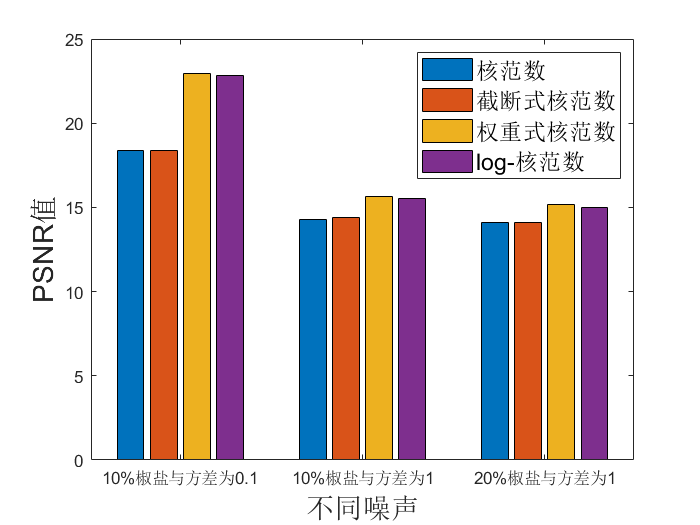
\includegraphics[scale=0.2]{exp-type-mixed.png}
\caption{不同的混合噪声}
\end{figure}
\end{frame}

\begin{frame}
\frametitle{\textbf{不同降噪方法的降噪效果}}
\begin{columns}
\column{.55\textwidth}
\begin{figure}
\centering
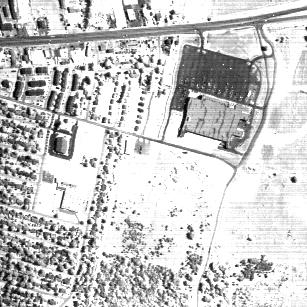
\includegraphics[scale=0.45]{band-103.jpg}
\caption{Urban数据集中一幅高光谱图像的第103个通道}
\label{band-103}
{\scriptsize{(数据来源:{\url{http://www.tec.army.mil/hypercube}})}}
\end{figure}

\column{.22\textwidth}
\begin{figure}
\centering
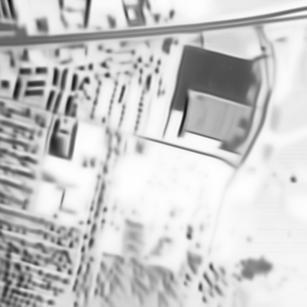
\includegraphics[scale=0.2]{band-103-NN.jpg}
\caption{对图\ref{band-103}运用核范数降噪}
\end{figure}
\begin{figure}
\centering
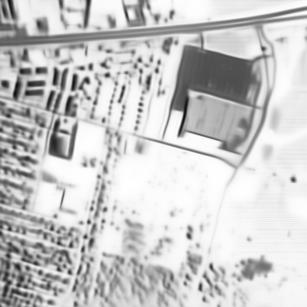
\includegraphics[scale=0.2]{band-103-WNN.jpg}
\caption{对图\ref{band-103}运用权重式核范数降噪}
\end{figure}

\column{.22\textwidth}
\begin{figure}
\centering
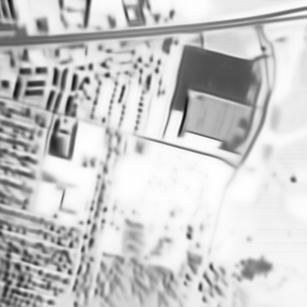
\includegraphics[scale=0.2]{band-103-TNN.jpg}
\caption{对图\ref{band-103}运用截断式核范数降噪}
\end{figure}
\begin{figure}
\centering
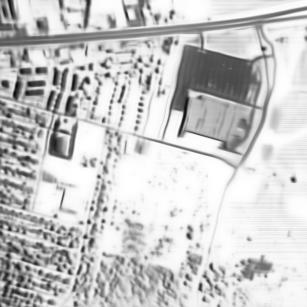
\includegraphics[scale=0.2]{band-103-LNN.jpg}
\caption{对图\ref{band-103}运用$log$-核范数降噪}
\end{figure}

\end{columns}
\end{frame}

\section[总结]{总结}
%\begin{frame}
%\frametitle{\textbf{总结}}
%	
%\end{frame}
\section[Q\&A]{Q\&A}
%\begin{frame}
%\frametitle{\textbf{Q\&A}}
%	
%\end{frame}
\section*{}
\begin{frame}
\begin{center}
\begin{minipage}{1\textwidth}
\setbeamercolor{mybox}{fg=white, bg=black!60!green}
\begin{beamercolorbox}[wd=0.70\textwidth, rounded=true, shadow=true]{mybox}
\LARGE \centering 感谢评委老师们的聆听!
\end{beamercolorbox}
\end{minipage}
\end{center}
\end{frame}
\end{document}
